% !TeX root = orbits.tex
% !TeX Program=pdfLaTeX

\chapter{The proofs by Feynman and Maxwell}\label{s.feynman}

Newton proved that if a planet is in an elliptical orbit around the Sun, as empirically determined by Kepler, it must be subject to the inverse-square law. Richard P. Feynman proved the converse: if a planet is subject to the inverse-square law then its orbit is elliptical. Using techniques similar to those later used by Feynman, James Clerk Maxwell proved Newton's theorem. Maxwell's proof was based on \emph{hodographs} which were previous used by William Rowan Hamilton to prove Newton's theorem.

\section{Dividing the orbit into sectors of equal angle}

Consider Kepler's second law (Figure~\ref{f.f-equal-area}). If the planet traverses both the long arc $\widehat{P_1P_2}$ and the short arc $\widehat{P_3P_4}$ in the same period of time, its speed during $\widehat{P_1P_2}$ must be greater than the speed during $\widehat{P_3P_4}$. The speed will be greatest at the planets closest approach to the Sun at $p$ (the \emph{perihelion}) and least at $a$ (the \emph{aphelion}).\footnote{These terms refer only to orbits about the Sun; for an arbitary orbit, the terms are \emph{periapsis} and \emph{apoapsis}.}

Feynman's approach was to divide the orbit not into sectors traversed in equal times, but into sectors of equal angles (Figure~\ref{f.f-equal-angles}). The planet will traverse the short arc $\widehat{P_1P_2}$ (near the perihelion) in a shorter time than long arc $\widehat{P_3P_4}$ (near the apehelion) so the areas of the sectors will not be equal.

%%%%%%%%%%%%%%%%%%%%%%%%%%%%%%%%%%%%%%%%%%%%%%%%%%%%%%%%%%%%%%%%

\begin{figure}
\begin{minipage}{.48\textwidth}
\begin{center}
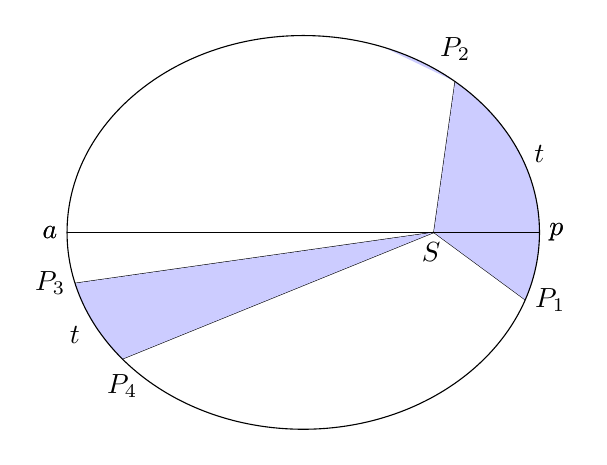
\begin{tikzpicture}
\clip (-3.5,-2.6) rectangle +(7,5.2);

% Size and center of the ellipse
\def\a{3}
\def\b{2.5}
\coordinate (O) at (0,0);

% Draw axis/axes through O
\coordinate (L) at (-180:{\a} and {\b});
\coordinate (R) at (0:{\a} and {\b});
\draw (L) -- (R);
\vertexsm{L};
\vertexsm{R};
\node[right] at (R) {$p$};
\node[left] at (L) {$a$};
 
% The Sun is at a focus
\coordinate (Sun) at ({+sqrt(\a*\a-\b*\b)},0);
\node[below,xshift=-1pt] at (Sun) {$S$};

% Locate and label four arbitrary points on the list
\coordinate (P1) at +(-20:{\a} and {\b});
\draw (P1) node[right] {$P_1$} -- (Sun);
\coordinate (P2) at +(50:{\a} and {\b});
\draw (P2) node[above,yshift=4pt] {$P_2$} -- (Sun);
\coordinate (P3) at +(195:{\a} and {\b});
\draw (P3) node[left] {$P_3$} -- (Sun);
\coordinate (P4) at +(220:{\a} and {\b});
\draw (P4) node[below,yshift=-2pt] {$P_4$} -- (Sun);

% Shade the sectors
\fill[blue!20] (Sun) -- (P1) arc [start angle = -20, end angle = 70,
    x radius = \a, y radius = \b] -- (P2) -- cycle;
\fill[blue!20] (Sun) -- (P3) arc [start angle = 195, end angle = 220,
    x radius = \a, y radius = \b] -- (P4) -- cycle;

% Draw the ellipse and bullets for the points
%   over the shade
\draw (0,0) ellipse({\a} and {\b});
\vertexsm{Sun};

% Label the times and areas
\node at (3,1) {$t$};
\node at (-2.9,-1.3) {$t$};

\draw (L) -- (R);
\vertexsm{L};
\vertexsm{R};
\node[right] at (R) {$p$};
\node[left] at (L) {$a$};

\end{tikzpicture}
\caption{Equal areas in equal times}\label{f.f-equal-area}
\end{center}
\end{minipage}
%%%%%%%%%%%%%%
\begin{minipage}{.48\textwidth}
\begin{center}
\begin{tikzpicture}
\clip (-3.5,-2.6) rectangle +(7,5.2);

% Size and center of the ellipse
\def\a{3}
\def\b{2.5}
\coordinate (O) at (0,0);

% Draw axis/axes through O
\coordinate (L) at (-180:{\a} and {\b});
\coordinate (R) at (0:{\a} and {\b});
%\draw (L) -- (R);

% Draw the ellipse and bullets for the points
%   over the shade
\draw[name path=ellipse] (0,0) ellipse({\a} and {\b});

% The Sun is at a focus
\coordinate (Sun) at ({+sqrt(\a*\a-\b*\b)},0);
\node[below] at (Sun) {$S$};
\node[right,xshift=5pt,yshift=1pt] at (Sun) {$\alpha$};
\node[left,xshift=-4pt,yshift=-1pt] at (Sun) {$\alpha$};
\vertexsm{Sun};

\path[name path=p1] (Sun) -- +(-20:2);
\path[name path=p2] (Sun) -- +(30:2);
\path[name path=p3] (Sun) -- +(160:5);
\path[name path=p4] (Sun) -- +(210:5);

\path [name intersections = {of = ellipse and p1, by = {P1} }];
\path [name intersections = {of = ellipse and p2, by = {P2} }];
\path [name intersections = {of = ellipse and p3, by = {P3} }];
\path [name intersections = {of = ellipse and p4, by = {P4} }];

\draw (P1) -- (P3);
\draw (P2) -- (P4);

\node[right,yshift=-2pt] at (P1) {$P_1$};
\node[right] at (P2) {$P_2$};
\node[left,yshift=3pt] at (P3) {$P_3$};
\node[below,xshift=-2pt] at (P4) {$P_4$};

\end{tikzpicture}
\caption{Equal angles}\label{f.f-equal-angles}
\end{center}
\end{minipage}
\end{figure}

%%%%%%%%%%%%%%%%%%%%%%%%%%%%%%%%%%%%%%%%%%%%%%%%%%%%%%%%%%%%%%%%

\begin{theorem}\label{thm.f-proportional}
The area of a sector is proportional to the square of the distance of a planet from the Sun.
\end{theorem}

\begin{proof}
Figure~\ref{f.f-similar-triangles} shows two sectors with the same central angle $\alpha$ approximated by triangles $\triangle P_1SP_2$ and $\triangle P_3SP_4$. Since the central angles are the same, we can ``overlay'' $\triangle P_1SP_2$ on $\triangle P_3SP_4$ to form $\triangle P_1'SP_2'$ (red).

Draw a line $P_3'P_4'$ parallel to $P_1'P_2'$ (blue) such that $A_{\triangle P_3'SP_4'}$, the area of $\triangle P_3'SP_4'$, equals $A_{\triangle P_3 SP_4}$. The dotted lines (green) show that by continuity such a line must exist. Since $P_1'P_2'\parallel P_3'P_4'$, $\triangle P_1'SP_2'\sim \triangle P_3'SP_4'$ and the sides of the triangles are proportional, $P_3'P_4'/P_1'P_2' = k$, as are the heights $h_{34}/h_{12}=k$. It follows that $A_{\triangle P_3'SP_4'}=k^2 A_{\triangle P_1'SP_2'}$. As the angle approaches zero, the triangles approach the sectors and the heights of the triangles approach the distance from the Sun to a position on the orbit.
\hqed 
\end{proof}

%%%%%%%%%%%%%%%%%%%%%%%%%%%%%%%%%%%%%%%%%%%%%%%%%%%%%%%%%%%%%%%%

\begin{figure}[t]
\begin{center}
\begin{tikzpicture}[scale=1.6]
\clip (-2.7,-.3) rectangle +(6.2,4);

% Size and center of the ellipse
\def\a{3}
\def\b{2.5}
\coordinate (O) at (0,0);

% Draw axis/axes through O
\coordinate (L) at (-180:{\a} and {\b});
\coordinate (R) at (0:{\a} and {\b});

% Draw the ellipse and bullets for the points
%   over the shade
\path[name path=ellipse] (0,0) ellipse({\a} and {\b});

% The Sun is at a focus
\coordinate (Sun) at ({+sqrt(\a*\a-\b*\b)},0);
\node[below] at (Sun) {$S$};
\vertexsm{Sun};

\path[name path=p1] (Sun) -- +(15:2);
\path[name path=p2] (Sun) -- +(55:2);
\path[name path=p3] (Sun) -- +(120:5);
\path[name path=p4] (Sun) -- +(160:6);

\path [name intersections = {of = ellipse and p1, by = {P1} }];
\path [name intersections = {of = ellipse and p2, by = {P2} }];
\path [name intersections = {of = ellipse and p3, by = {P3} }];
\path [name intersections = {of = ellipse and p4, by = {P4} }];

\draw[dashed,name path=extension] (Sun) --  ($(Sun)!1.5!(P3)$); 
\draw (Sun) -- (P1) -- (P2) -- (Sun) -- (P3) -- (P4) -- cycle;

\node[right,yshift=-2pt] at (P1) {$P_1$};
\node[right] at (P2) {$P_2$};
\node[right,yshift=3pt] at (P3) {$P_3$};
\node[below,xshift=-2pt] at (P4) {$P_4$};

\draw[red,thick] ($(Sun)!1!105:(P2)$) coordinate (P2P) 
  node[black,below] {$P_2'$} -- 
  (Sun) -- ($(Sun)!1!105:(P1)$) coordinate (P1P)
  node[black,right] {$P_1'$} -- cycle;

\path[name path=one] (P4) -- +(40:4);
\path[name path=two] ($(Sun)!.87!(P4)$) coordinate (x2) -- +(40:3.5);
\path[name path=three] (P3) -- +(220:3);

\path [name intersections = {of = extension and one,   by = {X1} }];
\path [name intersections = {of = extension and two,   by = {X2} }];
\path [name path=extension1] (Sun) -- (P4);
\path [name intersections = {of = extension1 and three, by = {X3} }];

\draw[very thick,dotted,green!70!black] (P4) -- (X1);
\draw[very thick,dotted,green!70!black] (P3) -- (X3);

\draw (P3) -- (P4);
\draw[thick,blue] (x2) node[black,below] {$P_4'$} --
  (X2) node[right,black] {$P_3'$};

\draw[thick,dashed,red] (Sun) -- node[black,below,near end,xshift=-6pt]
  {\sm{h_{12}}} ($(P1P)!(Sun)!(P2P)$);
\draw[thick,dashed,blue] (Sun) -- node[black,below,near end,xshift=-6pt] 
  {\sm{h_{34}}} ($(x2)!(Sun)!(X2)$);

\node[above right,xshift=4pt,yshift=1pt] at (Sun) {$\alpha$};
\node[above left,xshift=-8pt,yshift=4pt] at (Sun) {$\alpha$};

\end{tikzpicture}
\caption{The area is proportional to the square of the distance}\label{f.f-similar-triangles}
\end{center}
\end{figure}

%%%%%%%%%%%%%%%%%%%%%%%%%%%%%%%%%%%%%%%%%%%%%%%%%%%%%%%%%%%%%%%%

\begin{theorem}\label{thm.deltav}
For sectors whose angle is $\alpha$, the change in velocity $\Delta v$ is independent of $r$, the distance of the planet from the Sun!
\end{theorem}
\begin{proof}
We have the following proportionalities.
\begin{center}
\begin{tabular}{l@{\hspace{3em}}l}
$\Delta A \sim \Delta t$ &  Kepler's second law\\
$\Delta A \sim r^2$ &Theorem~\ref{thm.f-proportional}\\
$F \sim 1/r^2$& Inverse-square law\\
$F  \sim  \Delta v / \Delta t$& Newton's second law
\end{tabular}
\end{center}
Together we get
\[
\Delta v \sim F \:\Delta t \sim F \:\Delta A \sim \frac{1}{r^2} \cdot r^2 = 1\,.\fqed
\]
\end{proof}

While Newton divided the orbit into sectors of equal time (Figure~\ref{f.grav-small}), Feynman divided the orbit into sectors of equal angle (Figure~\ref{f.f-orbit}). By separating the motion along the orbit into unaccelerated motion continuing from the previous sector, followed by accelerated motion towards the Sun with the same direction as at the start of the sector, the diagrams look similar. By theorem Theorem~\ref{thm.deltav}, changes in velocity are of equal magnitude.

%%%%%%%%%%%%%%%%%%%%%%%%%%%%%%%%%%%%%%%%%%%%%%%%%%%%%%%%%%%%%%%%

\section{The velocity circle}

We now extract the velocity vectors from the orbit diagram (Figure~\ref{f.f-velocity}). Since vectors only have a direction and magnitude, not a position, we can reposition the vectors to have a common origin (Figure~\ref{f.f-exterior-angles}). The next theorem shows that the exterior angles are equal, from which we can deduce that $\Delta v$ vectors (all of which are equal) form a regular polygon.

%%%%%%%%%%%%%%%%%%%%%%%%%%%%%%%%%%%%%%%%%%%%%%%%%%%%%%%%%%%%%%%%%

\begin{figure}
\begin{minipage}{.48\textwidth}
\begin{center}
\begin{tikzpicture}[scale=1.6]
\clip (1.3,-.5) rectangle +(3,4.2);

% Size and center of the ellipse
\def\a{3.5}
\def\b{3}
\coordinate (O) at (0,0);

\draw[name path=ellipse] (O) ellipse({\a} and {\b});
\coordinate (S) at ({+sqrt(\a*\a-\b*\b)},0);
\node[below left] at (S) {$S$};
\vertexsm{S};

% Locate and label three arbitrary points on the list
\path [name path=z] (S) -- ($(S)+(-45:2.5)$);
\path [name intersections = {of = ellipse and z, by = {Z} }];
%\draw (S) -- (Z) node[right] {$Z$};
\path [name path=a] (S) -- ($(S)+(-10:2.5)$);
\path [name intersections = {of = ellipse and a, by = {A} }];
\draw (S) -- (A) node[right] {$A$};
\path [name path=b] (S) -- ($(S)+(25:2.5)$);
\path [name intersections = {of = ellipse and b, by = {B} }];
\draw (S) -- (B) node[above right,xshift=-2pt] {$B$};
\path [name path=c] (S) -- ($(S)+(60:2.5)$);
\path [name intersections = {of = ellipse and c, by = {C} }];
\draw (S) -- (C) node[left,yshift=-4pt] {$C$};
\path [name path=d] (S) -- ($(S)+(95:3)$);
\path [name intersections = {of = ellipse and d, by = {D} }];
\draw (S) -- (D) node[right,xshift=4pt,yshift=2pt] {$D$};

\path[name path=za] (Z) -- ($(Z) ! 2 ! (A)$);
\path[name path=b] (B) -- +(-10:1.5);
\path [name intersections = {of = za and b, by = {BP} }];
\vertexsm{BP};
\draw[thick,dashed] (A) -- (BP) node[right] {$B'$};
\draw[very thick,dashed,red,->] (BP) -- 
  node[above,xshift=8pt] {$\bm{\Delta v}$} (B);

\path[name path=ab] (A) -- ($(A) ! 3 ! (B)$);
\path[name path=c] (C) -- +(25:2);
\path [name intersections = {of = ab and c, by = {CP} }];
\vertexsm{CP};
\draw[thick,dashed] (B) -- (CP) node[above right] {$C'$};
\draw[very thick,dashed,red,->] (CP) -- 
  node[above,yshift=2pt] {$\bm{\Delta v}$} (C);

\path[name path=bc] (B) -- ($(B) ! 3 ! (C)$);
\path[name path=d] (D) -- +(60:1);
\path [name intersections = {of = bc and d, by = {DP} }];
\vertexsm{DP};
\draw[thick,dashed] (C) -- (DP) node[above right] {$D'$};
\draw[very thick,red,dashed,->] (DP) -- 
  node[near start,left] {$\bm{\Delta v}$} (D);
\draw (A) -- (B) -- (C) -- (D);

\node[right,xshift=10pt,yshift=2pt] at (S) {$\alpha$};
\node[above right,xshift=6pt,yshift=5pt] at (S) {$\alpha$};
\node[above,xshift=4pt,yshift=10pt] at (S) {$\alpha$};

\end{tikzpicture}
\caption{Orbit diagram}\label{f.f-orbit}
\end{center}
\end{minipage}
%%%%%%%%%%%%%%%%%%%%%%%%%%%%%%%%%%%%%%%%%%%%%%%%%%%%%%%%%%%%%%%%%
\begin{minipage}{.48\textwidth}
\begin{center}
\begin{tikzpicture}[scale=1.6]
\clip (1.3,-.5) rectangle +(3,4.2);

% Size and center of the ellipse
\def\a{3.5}
\def\b{3}
\coordinate (O) at (0,0);

\path[name path=ellipse] (O) ellipse({\a} and {\b});
\coordinate (S) at ({+sqrt(\a*\a-\b*\b)},0);

% Locate and label three arbitrary points on the list
\path [name path=z] (S) -- ($(S)+(-45:2.5)$);
\path [name intersections = {of = ellipse and z, by = {Z} }];
\path (S) -- (Z);
\path [name path=a] (S) -- ($(S)+(-10:2.5)$);
\path [name intersections = {of = ellipse and a, by = {A} }];
\path (S) -- (A) node[left] {$A$};
\path [name path=b] (S) -- ($(S)+(25:2.5)$);
\path [name intersections = {of = ellipse and b, by = {B} }];
\path (S) -- (B) node[left,xshift=0pt] {$B$};
\path [name path=c] (S) -- ($(S)+(60:2.5)$);
\path [name intersections = {of = ellipse and c, by = {C} }];
\path (S) -- (C) node[left,yshift=-4pt] {$C$};
\path [name path=d] (S) -- ($(S)+(95:3)$);
\path [name intersections = {of = ellipse and d, by = {D} }];
\path (S) -- (D) node[below,xshift=-2pt,yshift=0pt] {$D$};

\path[name path=za] (Z) -- ($(Z) ! 2 ! (A)$);
\path[name path=b] (B) -- +(-10:1.5);
\path [name intersections = {of = za and b, by = {BP} }];
\draw[->] (A) -- (BP) node[right] {$B'$};
\draw[->] (BP) -- node[above,xshift=5pt] {$\Delta v$} (B);

\path[name path=ab] (A) -- ($(A) ! 3 ! (B)$);
\path[name path=c] (C) -- +(25:2);
\path [name intersections = {of = ab and c, by = {CP} }];
\draw[->] (B) -- (CP) node[above right] {$C'$};
\draw[->] (CP) -- node[above,yshift=2pt] {$\Delta v$} (C);

\path[name path=bc] (B) -- ($(B) ! 3 ! (C)$);
\path[name path=d] (D) -- +(60:1);
\path [name intersections = {of = bc and d, by = {DP} }];
\draw[->] (C) -- (DP) node[above right] {$D'$};
\draw[->] (DP) -- node[near start,left] {$\Delta v$} (D);

\end{tikzpicture}
\caption{Velocity vectors}\label{f.f-velocity}
\end{center}
\end{minipage}
\end{figure}

%%%%%%%%%%%%%%%%%%%%%%%%%%%%%%%%%%%%%%%%%%%%%%%%%%%%%%%%%%%%%%%%%

\begin{figure}[b]
\begin{minipage}{.48\textwidth}
\begin{center}
\begin{tikzpicture}[scale=4.05]
\clip (2.4,-.5) rectangle +(1.5,1.62);

% Size and center of the ellipse
\def\a{3.5}
\def\b{3}
\coordinate (O) at (0,0);

\path[name path=ellipse] (O) ellipse({\a} and {\b});
\coordinate (S) at ({+sqrt(\a*\a-\b*\b)},0);

% Locate and label three arbitrary points on the list
\path [name path=z] (S) -- ($(S)+(-45:2.5)$);
\path [name intersections = {of = ellipse and z, by = {Z} }];
\path [name path=a] (S) -- ($(S)+(-10:2.5)$);
\path [name intersections = {of = ellipse and a, by = {A} }];
\path [name path=b] (S) -- ($(S)+(25:2.5)$);
\path [name intersections = {of = ellipse and b, by = {B} }];
\path [name path=c] (S) -- ($(S)+(60:2.5)$);
\path [name intersections = {of = ellipse and c, by = {C} }];
\path [name path=d] (S) -- ($(S)+(95:3)$);
\path [name intersections = {of = ellipse and d, by = {D} }];

\path[name path=za] (Z) -- ($(Z) ! 2 ! (A)$);
\path[name path=b] (B) -- +(-10:1.5);
\path [name intersections = {of = za and b, by = {BP} }];
\draw (BP) -- node[below,xshift=0pt] {$\Delta v$} (B);
\draw[thick,red] (B) node[black,above] {$B/C'$} -- +($(B)-(BP)$);

\path[name path=ab] (A) -- ($(A) ! 3 ! (B)$);
\path[name path=cpath] (C) -- +(25:2);
\path [name intersections = {of = ab and cpath, by = {CP} }];
\draw[thick,red] (B) -- node[black,below,xshift=2pt,yshift=-2pt] 
  {$\Delta v$} +($(C)-(CP)$) coordinate (c);
\draw[thick,blue] (c) -- +($(C)-(CP)$);

\path[name path=bc] (B) -- ($(B) ! 3 ! (C)$);
\path[name path=dpath] (D) -- +(60:1);
\path [name intersections = {of = bc and dpath, by = {DP} }];
\draw[thick,blue] (c) -- node[black,right,yshift=0pt] 
  {$\Delta v$} +($(D)-(DP)$) coordinate (d);
\node[above] at (c) {$C/D'$};
\node[left] at (d) {$D$};
\draw[->] (A) -- (B);
\draw[->] (A) -- (c);
\draw[->] (A) -- (d);
\draw[->] (A) -- (BP) node[above] {$B'$};
\end{tikzpicture}
\caption{Exterior angles}\label{f.f-exterior-angles}
\end{center}
\end{minipage}
%%%%%%%%%%%%%%%%%%%%%%%%%%%%%%%%%%%%%%%%%%%%%%%%%%%%%%%%%%%%%%%%%
\begin{minipage}{.48\textwidth}
\begin{center}
\begin{tikzpicture}[scale=1.5]
\clip (-.2,-.5) rectangle +(4.4,4.4);

% Size and center of the ellipse
\def\a{3.5}
\def\b{3}
\coordinate (O) at (0,0);

\draw[name path=ellipse] (O) ellipse({\a} and {\b});
\coordinate (S) at ({+sqrt(\a*\a-\b*\b)},0);
\node[below left] at (S) {$S$};
\vertexsm{S};

% Locate and label three arbitrary points on the list
\path [name path=z] (S) -- ($(S)+(-45:2.5)$);
\path [name intersections = {of = ellipse and z, by = {Z} }];
\path [name path=a] (S) -- ($(S)+(-10:2.5)$);
\path [name intersections = {of = ellipse and a, by = {A} }];
\draw (S) -- (A) node[right] {$A$};
\path [name path=b] (S) -- ($(S)+(25:2.5)$);
\path [name intersections = {of = ellipse and b, by = {B} }];
\draw (S) -- (B) node[above right,xshift=-2pt] {$B$};
\path [name path=c] (S) -- ($(S)+(60:2.5)$);
\path [name intersections = {of = ellipse and c, by = {C} }];
\draw (S) -- (C) node[left,xshift=-4pt,yshift=0pt] {$C$};
\path [name path=d] (S) -- ($(S)+(95:3)$);
\path [name intersections = {of = ellipse and d, by = {D} }];
\draw (S) -- (D) node[right,xshift=4pt,yshift=2pt] {$D$};

\path[name path=za] (Z) -- ($(Z) ! 2 ! (A)$);
\path[name path=b] (B) -- +(-10:1.5);
\path [name intersections = {of = za and b, by = {BP} }];
\draw[thick] (A) -- (BP) node[right] {$B'$};
\draw[very thick,red,->] (BP) -- node[above,xshift=8pt] 
  {$\bm{\Delta v}$} (B);

\draw[blue,thick] (B) -- +($(B)-(BP)$) coordinate (bbp);
\draw[blue,thick] (B) -- ($(B)!8!(bbp)$);

\path[name path=ab] (A) -- ($(A) ! 3 ! (B)$);
\path[name path=c] (C) -- +(25:2);
\path [name intersections = {of = ab and c, by = {CP} }];
\draw[thick] (B) -- (CP) node[above right] {$C'$};
\draw[very thick,red,->] (CP) -- node[above,yshift=2pt] 
  {$\bm{\Delta v}$} (C);

\draw[blue,thick] (C) -- +($(C)-(CP)$) coordinate (ccp);
\draw[blue,thick,name path=ccpath] (C) -- ($(C)!7!(ccp)$);

\path[name path=bc] (B) -- ($(B) ! 3 ! (C)$);
\path[name path=d] (D) -- +(60:1);
\path [name intersections = {of = bc and d, by = {DP} }];
\draw[thick] (C) -- (DP) node[above right] {$D'$};
\draw[very thick,red,->] (DP) -- node[near start,left] 
  {$\bm{\Delta v}$} (D);

\draw[blue,thick] (D) -- +($(D)-(DP)$) coordinate (ddp);
\draw[blue,thick,name path=ddpath] (D) -- ($(D)!5!(ddp)$);

\path [name intersections = {of = ccpath and ddpath, by = {X} }];
\node[above,xshift=-4pt] at (X) {$X$};
\draw (A) -- (B) -- (C) -- (D);

\node[right,xshift=10pt,yshift=2pt] at (S) {$\alpha$};
\node[above right,xshift=6pt,yshift=5pt] at (S) {$\alpha$};
\node[above,xshift=4pt,yshift=10pt] at (S) {$\alpha$};

\node[below,xshift=-3pt,yshift=-10pt] at (D) {$\alpha$};
\node[below left,xshift=-6pt,yshift=-6pt] at (C) {$\alpha$};
\node[above right,xshift=6pt,yshift=6pt] at (X) {$\alpha$};

\end{tikzpicture}
\caption{Equality of the exterior angles}\label{f.f-circle}
\end{center}
\end{minipage}
\end{figure}

%%%%%%%%%%%%%%%%%%%%%%%%%%%%%%%%%%%%%%%%%%%%%%%%%%%%%%%%%%%%%%%%

\begin{theorem}
The exterior angles of the velocity diagram are equal.
\end{theorem}
\begin{proof}
Figure~\ref{f.f-circle} is taken from the orbit diagram (Figure~\ref{f.f-orbit}) with the $\Delta v$ vectors extended. Let $X$ be he intersection of $CC'$ and $DD'$. By construction $CX\parallel BS$ and $DX\parallel CS$. Since the angles at $S$ are equal ($\alpha$), by alternate interior angles, the angles at $C,D,X$  are equal. Since $\angle CXD=\alpha$, so is its vertical angle which is the exterior angle between $C'C$ and $D'D$ (examine Figure~\ref{f.f-exterior-angles}), and it follows that all exterior angles are equal.\fqed
\end{proof}

Consider the polygon whose sides are formed by the $\Delta v$ vectors for all sectors of the orbit. Since the exterior angles are equal, the polygon is regular, and as the number of sectors increases, the polygon approaches  the ``velocity circle.''

%%%%%%%%%%%%%%%%%%%%%%%%%%%%%%%%%%%%%%%%%%%%%%%%%%%%%%%%%%%%%%%%

\begin{figure}
\begin{center}
\begin{tikzpicture}[scale=.85]
\clip (-4,-1.5*2.5-.1) rectangle +(8,3.3*2.4);
\coordinate (C) at (0,0);
\draw (C) circle [radius=3.8cm];
\coordinate (O) at (1.6,1);
\vertexsm{O};
\draw (3.8,0)
\foreach \angle in {30,60,...,360} {
  -- node[fill=white] {\sm{\Delta v}} (\angle:3.8)
};
\foreach \angle in {0,30,...,360} {
  \draw[->] (O) -- (\angle:3.8);
};
\end{tikzpicture}
\caption{Velocity circle}\label{f.f-velocity-circle}
\end{center}
\end{figure}

%%%%%%%%%%%%%%%%%%%%%%%%%%%%%%%%%%%%%%%%%%%%%%%%%%%%%

\begin{figure}[b]
\begin{minipage}{.5\textwidth}
\begin{center}
\begin{tikzpicture}[scale=.885]

\clip (0,-1) rectangle +(5.7,5.6);
%\clip (-2.1,-2.1) rectangle +(4.3,4.5);

% Size and center of the ellipse
\def\a{4.5}
\def\b{3}
\def\angle{30}

\pic{semi-ellipse={\a}/{\b}};
\pic{point-on-ellipse={\a}/{\b}/{\angle}};
\pic{tangent-path={\a}/{\b}/{\angle}};
\node[below] at (F2) {$S$};
\node[above right] at (F2) {$\alpha$};
\draw (F2) -- (P);
\draw[->] (P) -- node[above] {$v_p$} ($(P)!.6!(R)$);
\draw[->] (Right) -- node[right] {$v_a$} +(90:2.5cm);
\node[right] at (Right) {$A$};

\end{tikzpicture}
\caption{The velocity is tangent to the orbit}\label{f.f-tangent}
\end{center}
\end{minipage}
%%%%%%%%%%%%%%%%%%%%%%%%%%%%%%%%%%%%%%%%%%%%%%%%%%%%%%%%%%%%%%%%
\begin{minipage}{.5\textwidth}
\begin{center}
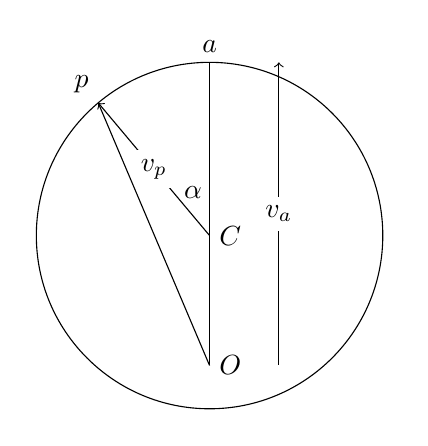
\begin{tikzpicture}[scale=1.1]

\clip (-2.1,-2.1) rectangle +(4.3,4.5);

\coordinate (C) at (0,0);
\vertexsm{C};
\node[right] at (C) {$C$};
\node[above,xshift=-6pt,yshift=10pt] at (C) {$\alpha$};
\coordinate (O) at (0,-1.5);
\node[right] at (O) {$O$};
\vertexsm{O};
\draw (C) circle[radius=2];
\draw (O) -- (0,2) node[above] {$a$};
\draw[->] (C) -- node[fill=white] {$v_p$} +(130:2) coordinate (p) node[above left] {$p$};
\draw (O) -- (p);

\draw[<-] (.8,2) -- node[fill=white] {$v_a$} (.8,-1.5);

\end{tikzpicture}
\caption{Vectors in the velocity circle}\label{f.f-vector-velocity}
\end{center}
\end{minipage}
\end{figure}

%%%%%%%%%%%%%%%%%%%%%%%%%%%%%%%%%%%%%%%%%%%%%%%%%%%%%%%%%%%%

We can now work with a smooth orbit and its velocity circle (Figures~\ref{f.f-tangent}, \ref{f.f-vector-velocity}). $v_a$ is the (tangential) velocity at the perihelion, so it will be the longest line from origin of circle to its circumference and must pass through the center of the circle. The velocity vectors are tangents to the orbit, and as the planet moves in the orbit, they remain so. Since the orbit has been divided into sectors of equal angle, the sectors of the velocity circle are also equal, and therefore $\angle ASP = \angle aCp=\alpha$.

The final step is to show that as $Cp$ rotates around the velocity circle, the orbit is an ellipse. In Figure~\ref{f.f-elliptical-orbit} let $p$ be an arbitrary point on the velocity circle with origin $O$ and center $C$.\footnote{For convenience the circle is rotated $90^\circ$ clockwise relative to the circle in Figure~\ref{f.f-vector-velocity}.} Construct the perpendicular bisector of $Op$ at $M$ and let its intersection with $Cp$ be $P$.

\newpage

\begin{theorem}
The locus of $P$ as $p$ moves around the velocity circle is an ellipse with foci $O,C$ and $OP+PC$ equals the radius of the circle.
\end{theorem}
\begin{proof}
$\triangle POM\cong \triangle PpM$ by side-angle-side, so $OP=Pp=x$ and $CP+PO=CP+Pp=Cp$ which is the radius of the circle and therefore constant for any choice of $p$.\fqed
\end{proof} 

Feynman found this to be the most difficult step to discover \cite[p.~130]{lost} although similar constructions can be found in theorems on ellipses such as Theorem~\ref{thm.tangent-angles}.

%%%%%%%%%%%%%%%%%%%%%%%%%%%%%%%%%%%%%%%%%%%%%%%%%%%%%%%%%%%%%%%%

\begin{figure}
\begin{center}
\begin{tikzpicture}[scale=1.8]

\clip (-2.1,-.4) rectangle +(4.5,2.5);

\coordinate (C) at (0,0);
\vertexsm{C};
\node[below] at (C) {$C$};
\coordinate (O) at (-1.1,0);
\node[below] at (O) {$O$};
\vertexsm{O};
\draw (C) circle[radius=2];
\draw (O) -- (2,0) node[right] {$a$};
\draw[name path=cp] (C) -- node[right] {$x$} +(50:2) 
  coordinate (p) node[above right] {$p$};
\draw (O) -- (p);

\coordinate (mid) at ($(O)!.5!(p)$);
\node[left,xshift=-2pt,yshift=2pt] at (mid) {$M$};

\draw[name path=perp] (mid) -- ($(mid)!.8!-90:(p)$);
\draw (mid) -- ($(mid)!.5!90:(p)$);
\draw[rotate=32] (mid) rectangle +(3pt,3pt);

\path [name intersections = {of = cp and perp, by = {P} }];
\node[right] at (P) {$P$};
\draw (O) -- node[below] {$x$} (P);
\path (C) -- node[right] {$y$} (P);
\end{tikzpicture}
\caption{The derivation of the inverse square law}\label{f.f-elliptical-orbit}
\end{center}
\end{figure}

%%%%%%%%%%%%%%%%%%%%%%%%%%%%%%%%%%%%%%%%%%%%%%%%%%%%%%%%%%%%%%%%

\section{Maxwell's proof}

Figure~\ref{f.maxwell} shows a construction similar to the one used in the proof of Theorem~\ref{thm.tangent-angles}. The foci are $S,H$, and $P,Q$ are points on the ellipse close to each other. Extend $SP$ to $SU$ so that its length is the same as the length of the major axis $AA'$. Bisect $HU$ at $Z$ and draw $ZP$ extended so that the perpendicular from $S$ to the line intersects it at $Y$. Theorem~\ref{thm.tangent-angles} showed that $ZP$ is a tangent to the ellipse and that $\angle HZP$ is a right angle.

The area swept out from $P$ to $Q$ is approximately that of the triangle $\triangle PSQ$ whose area is $\frac{1}{2}PQ\cdot SY$ since $SY$ is the height of the triangle. The velocity at $P$ is $v=PQ/\Delta t$ so
\[
\kappa = \frac{\Delta A}{\Delta t} = \frac{\frac{1}{2}PQ\cdot SY}{\Delta t} = \frac{1}{2}v SY\,.
\]
By Theorem~\ref{thm.perp-perp-tangent}, $SY\cdot HZ=BC^2$.
\begin{eqnarray*}
HU&=& 2HZ = \frac{2BC^2}{SY}\\
&=& \frac{2BC^2}{2\kappa/v}\\
v &=& \frac{\kappa HU}{BC^2}\,.
\end{eqnarray*}
We conclude that $HU$ is perpendicular to the velocity vector at $P$ and proportional to the vector. Similarly, for $HV$, the line from $H$ to $V$, the extension of $SQ$, and for any other point on the ellipse. Therefore, the lines $SU, SV, \ldots$ are all equal to $AA'$, creating the velocity  circle with center $S$ and radius $r=AA'$.

By Theorem~\ref{thm.f-proportional}, 
\begin{eqnarray*}
\kappa&=&\frac{\Delta A}{\Delta t} \sim \frac{r^2}{\Delta t}\\
a&=&\frac{\Delta v}{\Delta t}= \frac{\kappa \Delta v}{r^2}\,.
\end{eqnarray*}
By Theorem~\ref{thm.deltav}, $\Delta v$ is independent of $r$, so the acceleration and hence the force to the focus $S$ is proportional to the inverse square of the distance.

%%%%%%%%%%%%%%%%%%%%%%%%%%%%%%%%%%%%%%%%%%%%%%%%%%%%%%%%%%%%%%%%

\begin{figure}[t]
\begin{center}
\begin{tikzpicture}[scale=.7]
\clip (-7,-6) rectangle +(14,13);

\def\a{5.25}
\def\b{3.5}
\def\angleP{20}
\def\angleQ{30}

\coordinate (O) at (0,0);
% Draw the ellipse
\draw[name path global=ellipse] (O) ellipse[x radius={\b},y radius={\a}];

% Locate foci
\coordinate (F1) at (0,{-sqrt(\a*\a-\b*\b)});
\coordinate (F2) at (0,{+sqrt(\a*\a-\b*\b)});
\node[left] at (F1) {$S$};
\node[left] at (F2) {$H$};

% Draw arc
\draw[name path=arc] ($(F1)+(130:{2*\a})$) 
  arc[start angle=130,end angle=50,radius={2*\a}];

% Locate vertices
\coordinate (Top) at (0,{\a});
\node[above left] at (Top) {$A'$};
\coordinate (Bot) at (0,{-\a});
\node[below left] at (Bot) {$A$};
\draw (Top) -- (Bot);

% Locate points on the ellipse
\coordinate (P) at ({\angleP}:{\b} and {\a});
\node[right] at (P) {$P$};
\coordinate (Q) at ({\angleQ}:{\b} and {\a});
\node[left] at (Q) {$Q$};
\draw (F2) -- (P);

% Locate points on circle
\path[name path=sp] (F1) -- ($(F1)!1.6!(P)$);
\path [name intersections = {of = arc and sp, by = {U} }];
\node[above right] at (U) {$U$};
\draw (F1) -- (U);
\path[name path=sq] (F1) -- ($(F1)!1.6!(Q)$);
\path [name intersections = {of = arc and sq, by = {V} }];
\draw (F1) -- (V) -- (F2);
\node[above] at (V) {$V$};

% Find Z
\draw (F2) -- (U);
\coordinate (Z) at ($(F2)!.5!(U)$);
\node[below right] at (Z) {$Z$};

% Find Y
\path[name path=zy] (Z) -- ($(Z)!3!(P)$);
\draw (F1) -- ($(Z)!(F1)!(P)$) coordinate (Y);
\draw (Y) -- (Z);
\node[right] at (Y) {$Y$};

\draw[rotate=105]  (Y) rectangle +(7pt,7pt);
\draw[rotate=195]  (Z) rectangle +(7pt,7pt);

\draw[thick,red] (F1) -- (P) -- (Q) -- cycle;

\end{tikzpicture}
\caption{Maxwell's proof}\label{f.maxwell}
\end{center}
\end{figure}

%%%%%%%%%%%%%%%%%%%%%%%%%%%%%%%%%%%%%%%%%%%%%%%%%%%%%%%%%%%%%%%%

\section{Hodographs}

A \emph{hodograph} is the curve traced out by the tips of velocity vectors of a trajectory or an orbit when their initial points are co-located. In Figure~\ref{f.f-exterior-angles} the path $B'BCD$ is a hodograph as is the regular polygon in Figure~\ref{f.f-velocity-circle}. The circle containing $U,V$ is a hodograph in Figure~\ref{f.maxwell}. This hodograph is instructive because it clearly shows how it is created by the velocity vectors starting at the focus $S$.

Hodographs were first proposed by William Rowan Hamilton who used them to prove Newton's theorem \cite{hamilton}. The advantage of hodographs is that velocity is a first-order derivative of position, while acceleration is a second-order derivative. Here we show that a hodograph can be used to easily obtain the horizontal distance traversed by a particle thrown at an angle and subject only to the force of gravity (Figure~\ref{f.hodograph1}).

%%%%%%%%%%%%%%%%%%%%%%%%%%%%%%%%%%%%%%%%%%%%%%%%%%%%%%%%%%%%%%%%

\begin{figure}[t]
\begin{center}
\begin{minipage}{.45\textwidth}
\begin{center}
\begin{tikzpicture}[scale=.8]
\path (-4,-1.8) rectangle +(8,1.8);
\draw (-4,0) parabola[bend pos=0.5] bend +(0,2) (4,0);
\draw[->] (-4,0) -- +(2,2) node[above] {$v_0$};
\draw[<-] (4,0) -- +(-2,2) node[above] {$v_f$};
\end{tikzpicture}
\caption{Path of a projectile}\label{f.hodograph1}
\end{center}
\end{minipage}
\hspace{3em}
\begin{minipage}{.45\textwidth}
\begin{center}
\begin{tikzpicture}
\draw[->] (0,0) node [above right,xshift=8pt] {$\theta$} -- 
  node[above left] {$v_0$} +(2,2);
\draw[->] (0,0) node [below right,xshift=8pt,yshift=1pt] {$\theta$} -- 
  node[below left] {$v_f$} +(2,-2);
\draw (2,2) -- node[right] {$gt$} (2,-2);
\draw[thick,dashed] (0,0) -- node[above,xshift=6pt] {$v_h$} ($(2,2)!(0,0)!(2,-2)$);
\end{tikzpicture}
\caption{Hodograph of a projectile}\label{f.hodograph2}
\end{center}
\end{minipage}
\end{center}
\end{figure}

The initial velocity is $v_0$ and the final velocity is $v_f$, where $|v_0|=|v_f|$. The hodograph is shown in Figure~\ref{f.hodograph2}. The horizontal component of the velocity is constant $v_h=v_0\cos \theta$, while the vertical velocity is $gt$, that is, it is proportional to the time until the particle hits the earth. Therefore, the area of the triangle,
\[
\frac{1}{2}v_h\cdot gt = \frac{1}{2}v_0\cos\theta \cdot gt
\]
is one-half the distance traversed by the particle.
